\documentclass[10pt, letterpaper, IEEEtran, tikz,border=5,a4paper,fleqn]{article}

\usepackage{algpseudocode}
\usepackage[margin=1in]{geometry}
%\renewcommand{\familydefault}{ppl}
\usepackage{tikz-qtree}

\usepackage{amsfonts, amsmath, amssymb, amsthm}
\usepackage{bm}
\usepackage{verbatim}
\usepackage{color}
\usepackage{euscript}
\usepackage{graphicx}
\usepackage[usenames,dvipsnames]{xcolor}
\usepackage{paralist}
\usepackage{mathtools}
\usepackage[demo]{graphicx}
\usepackage{subcaption}

\usepackage{algorithm}

\usepackage{multicol}
\usepackage{xspace}
\usepackage{wrapfig}
\usepackage{hyperref}
\usepackage{amsmath}

\def\figcapup{\vspace{-0mm}}
\def\figcapdown{\vspace{-0mm}}
\def\extraspacing{\vspace{2mm} \noindent}
\def\minilen{0.95\linewidth}
\def\vgap{\vspace{0.1 in}}

\def\S{\mathcal{S}}
\def\nil{\textsc{\em nil}}

\newcommand{\IR}{\mathbb{R}}
\newcommand{\olc}{\overline{c}}

\newcommand\tab[1][0.5cm]{\hspace*{#1}}
\newtheorem{theorem}{Theorem}
\newtheorem{lemma}{Lemma}
\newtheorem{corollary}{Corollary}
\newtheorem{observation}{Observation}
\newtheorem{proposition}{Proposition}
\newtheorem{definition}{Definition}
\newtheorem{problem}{Problem}

\definecolor{mygray}{gray}{0.4}

\graphicspath{ {images/} }

\begin{document}
%\begin{sloppy}
\title{\vspace{-1 in}E 0243: Assignment 1}

\date{ \vspace{-0.5 in} Aman Sachan (18094) \hspace{30mm} Paras Lohani (18226)}

\maketitle

% \paragraph{Instructions}
% \begin{itemize}
% \item Both the problems carry equal weight.
% \item Academic dishonesty/plagiarism will be dealt with severely.
% \item Late submissions are accepted only with prior approval or medical certificate.
% \end{itemize}

\section{Introduction}

CPI is cycle per instruction which symbolizes the number of cycles taken by an instruction. It depends on the cycles taken by the various hardware events. Each CPI contains a base CPI which reflects the minimum CPI needed to execute instructions. Since we are experimenting in a superscalar processor, there is a chance of overlapping of hardware events which will effect CPI accordingly. We will run experiment on various benchmarks to understand the performance of our processor and the impact of various hardware events on it.

\section{Hardware Performance Counters}
Hardware Performance Counters is a type of registers which stores the count of hardware related events performed in the computer systems.\\
We have done all the computations in the Intel(R) Core(TM) i3-6006U CPU @ 2.00GHz  processor for the following SPECINT Benchmarks \verb| 531.deepsjeng_r, 520.omnetpp_r, 557.xz_r| and for SPECFP Benchmarks \verb| 526.blender_r, 507.cactuBSSN_r, 511.povray_r|.

\subsection{Performace monitoring tool}

Open source tool named \verb|perf| has been used to collect supported hardware events counters on a given program. It gives facility of command line interface where one can use commands to collect, analyze performance and trace data. The \verb|perf| commands used are \verb|stat|, \verb|record|, \verb|report|, etc.

\subsection{Data Collection}

Using \verb|perf| we collected the measures of performance counters in the user space. The data is collected for atmost these following 11 events:-
\begin{multicols}{3}
\begin{itemize}
    \item \verb|cycles|
    \item \verb|instructions|
    \item \verb|branch-misses|
    \item \verb|L2-load-misses|
\end{itemize}
\columnbreak
\begin{itemize}
    \item \verb|L2-store-misses|
    \item \verb|L1-dcache-load-misses|
    \item \verb|L1-icache-load-misses|
    \item \verb|dTLB-load-misses|
\end{itemize}
\columnbreak
\begin{itemize}
    \item \verb|dTLB-store-misses|
    \item \verb|iTLB-load-misses|
    \item \verb|branch-load-misses|
\end{itemize}
\end{multicols}

\noindent We have used the command \\
\indent \verb|perf stat -I interval(in ms) -e cycles:u,instructions:u,branch-misses:u,|\\ \indent \verb|L1-dcache-load-misses:u,L1-icache-load-misses:u,dTLB-load-misses:u,dTLB-|\\ \indent \verb|store-misses:u,iTLB-load-misses:u,branch-load-misses:u,L2-load-misses:u,|\\ \indent \verb|L2-store-misses:u bash ./run.sh taskset--cpu-list 0 2>filename.txt|\\
to generate the dataset in the file and set the benchmark to run on only one core of the processor after that we have to pre-process it(data cleaning), to get data in proper format.

\subsection{Data Cleaning}

Data collected from the perf tool is in row format where each row depicts the counter information for a particular hardware events. Data in a row is in the form of [Time, Counter value, Event name]. These hardware events will be used as independent variables in our model, therefore pre-processing needs to be done on the data collected from the previous step to transform it to column format. The counters collected are comma separated which is not suitable for model creation, therefore some cleaning steps need to be performed on the dataset. While analysing values of columns we have observed some outliers which is removed. This outliers mainly has CPI way more than the mean CPI collected.

\subsection{Data Visualization}

Figure 1. shows the scatter plot of various events against CPI in the \verb|557.xz_r| benchmark. We can observe that there is a positive slope linear relationship of each events with the CPI. This conclude that all the events contribute in an additive fashion.

\begin{figure}
\begin{subfigure}{.33\textwidth}
  \centering
  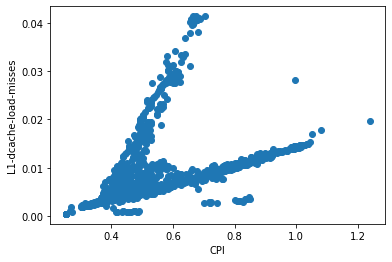
\includegraphics[width=.9\linewidth]{l1-dcache-load.png}

\end{subfigure}%
\begin{subfigure}{.33\textwidth}
  \centering
  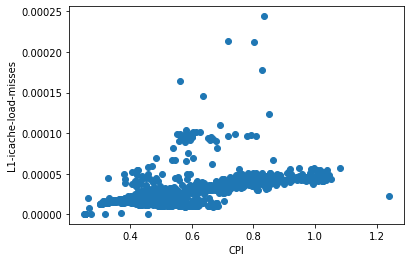
\includegraphics[width=.9\linewidth]{l1-icache-load.png}

\end{subfigure}%
\begin{subfigure}{.33\textwidth}
  \centering
  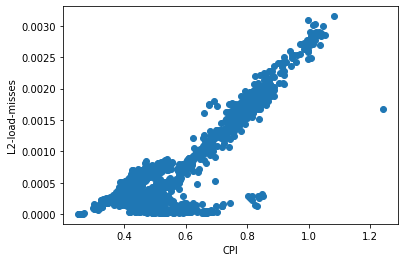
\includegraphics[width=.9\linewidth]{L2-load-misses.png}

\end{subfigure}

\begin{subfigure}{.33\textwidth}
  \centering
  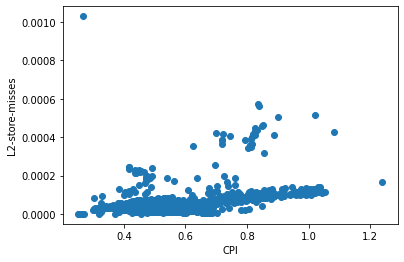
\includegraphics[width=.9\linewidth]{L2-store-misses.png}

\end{subfigure}%
\begin{subfigure}{.33\textwidth}
  \centering
  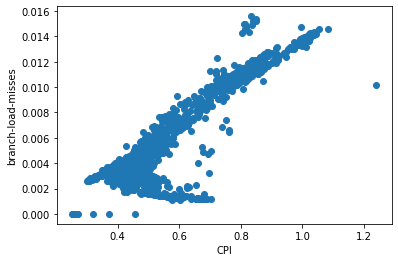
\includegraphics[width=.9\linewidth]{branch-load-misses.png}

\end{subfigure}%
\begin{subfigure}{.33\textwidth}
  \centering
  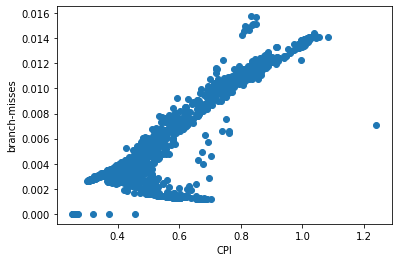
\includegraphics[width=.9\linewidth]{branch-misses.png}

\end{subfigure}
\begin{subfigure}{.33\textwidth}
  \centering
  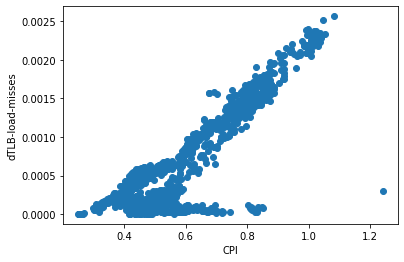
\includegraphics[width=.9\linewidth]{dTLB-load-misses.png}

\end{subfigure}%
\begin{subfigure}{.33\textwidth}
  \centering
  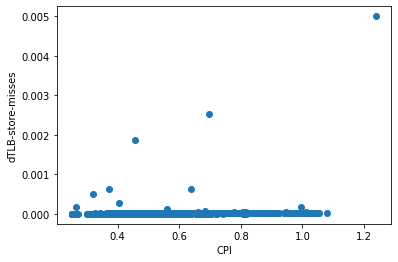
\includegraphics[width=.9\linewidth]{dTLB-store-misses.png}

\end{subfigure}%
\begin{subfigure}{.33\textwidth}
  \centering
  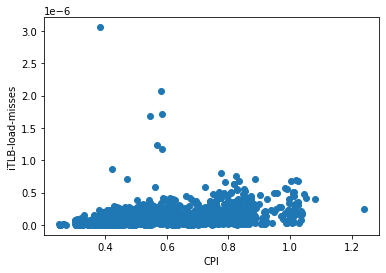
\includegraphics[width=.9\linewidth]{iTLB-load-misses.png}

\end{subfigure}
\caption{Various hardware events against CPI}
\label{fig:fig}
\end{figure}

\subsection{Basic Statistical Measures}

After cleaning data, we analyzed the distribution of data column wise. For each column we get the information like count, mean, std, min, max etc.\\

\noindent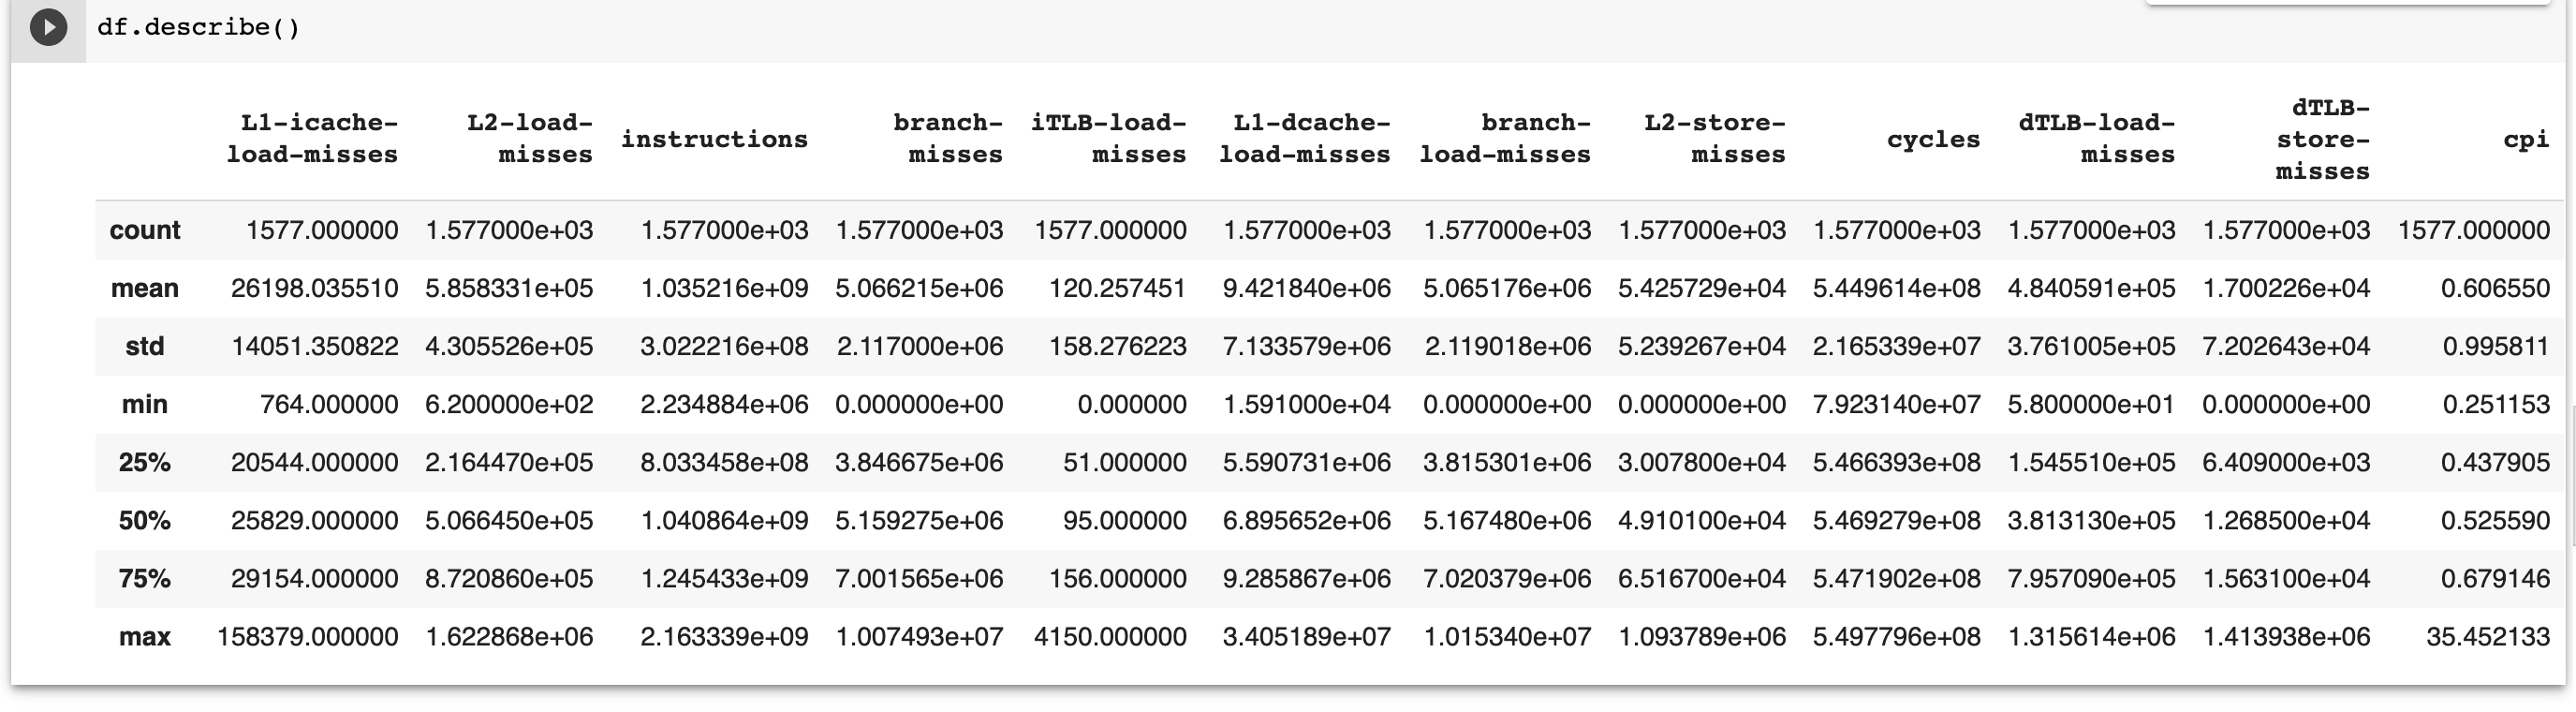
\includegraphics[scale=0.33]{Statistics.png}

\subsection{Normalization}

Instead of normalizing the data using traditional min-max, range-transformation etc., we are dividing the counters of various events with the corresponding instruction counter. This way we will deal with 0-1 data values.

\section{Learning Model using Linear Regression}

\subsection{Sampling}

As different benchmarks take different amount of running time. So, we have taken different intervals according to the running time of the benchmark. We have computed approx 1250+ datasets for each benchmark and trained our Linear Regression model on random 80\% of the datasets (1000+) and test it on the remaining 20\% of the datasets (250+) on average.

\subsection{Linear Regression}

We have used a Multiple Linear Regression model and a base as Linear Regression. To build the model we used \verb|python| and some already available python libraries such as \verb| numpy, matplotlib, statsmodels,|\\ \verb|pandas, sklearn, math, seaborn|.\\
To analyze the CPI stack i.e, how the features are impacting the CPI stack, we restricted our coefficients to be non-negative.

\subsection{Error Analysis}

We have used different error analyzing factor such as \verb| R2, Residuals, F-statistic, p-value,|\\ \verb|RMSE and Adjusted R2 values| to assess the quality of the model generated.

\section{Code}

Code is written in \textbf{Python} using \textbf{Google Colab}. For the preprocessing, one can refer \href{https://colab.research.google.com/drive/1VmkJbYE7EdJ5HFUyMy4FOpxf_3iagbxn?usp=sharing}{\color{blue} this link}. For the linear regression models, one can refer \href{https://colab.research.google.com/drive/1qcsSkg_DKaM5B8WkhQnJwOg_wozr9eaJ?usp=sharing}{\color{blue} this link}. \href{https://colab.research.google.com/drive/1AYyh_fw5Jp6La6UNAu6Yj63GjWdVIcUc?usp=sharing}{Final code} having all the code that can be run on all the benchmarks for the cpi stack creation.

\section{Results}

CPI Stack(dependent variable) is computed on our test hardware events using our trained Linear Regression model. This model uses the equation :- \[y = \beta_0 + \beta_1*x_1 + \beta_2*x_2 + ...\]
where, $y$ will be estimated CPI, $\beta_0$ is base CPI, $\beta_i$ is the coefficient corresponding to the feature $x_i$.\\
Coefficients is representing the number of cycles required for a particular miss event and the factors are in the term of number of miss events per instruction.

\begin{figure}[h]
 \begin{center}
      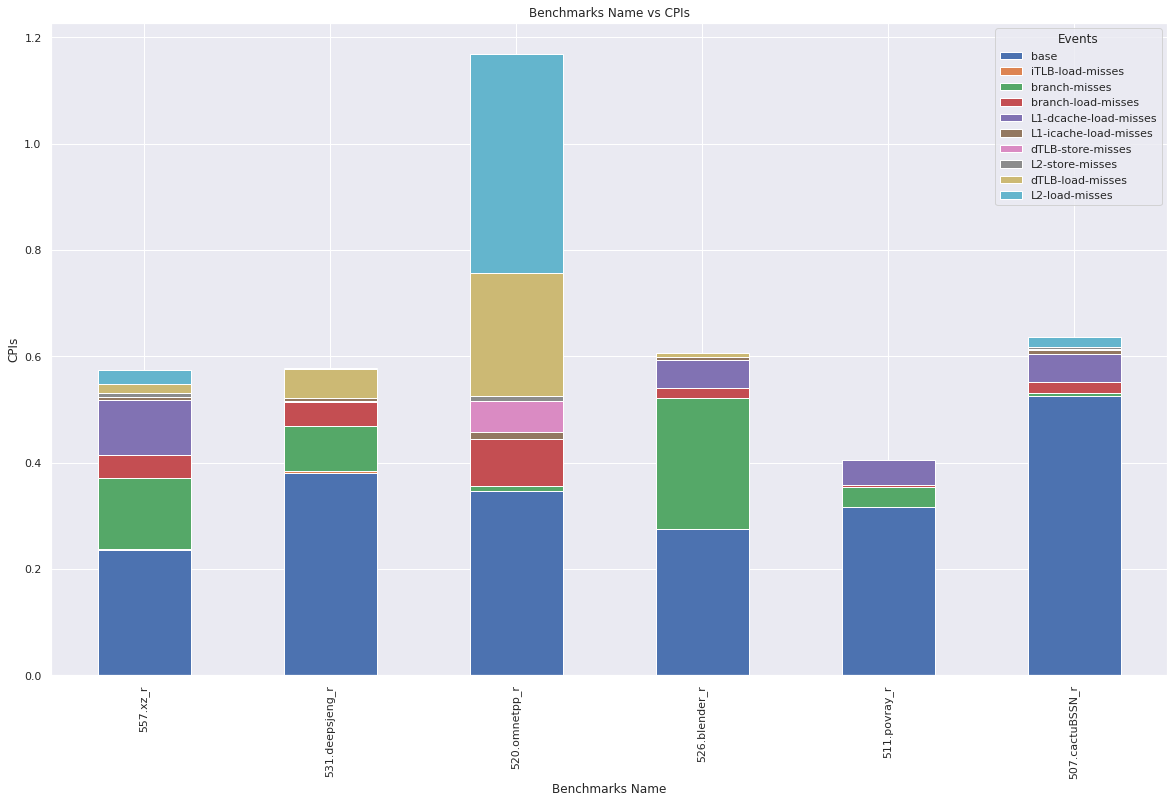
\includegraphics[scale=.37]{cpi_stack.png}
 \end{center}
 \label{fig:cpi_stack}
\end{figure}

\subsection{SPECINT Benchmarks}

\subsubsection{557.xz\_r}

Number of dataset are 1575 and we trained on random 80\% of the dataset. We have taken the interval to be 275 ms and run our model on whole interval.
\begin{center}
\begin{tabular}{||c c c c||}
 \hline
 \textbf{events} & \textbf{mean} & \textbf{coefficients} & \textbf{p-value}\\ [0.5ex]
 \hline\hline
 L1-icache-load-misses & 2.8024535566934098e-05 & 180.78003596543587 & 0.000\\
 \hline
 dTLB-load-misses & 0.0005953550353532326 & 32.26056892641485 & 0.009\\
 \hline
 iTLB-load-misses & 1.2934668363220614e-07 & 8796.132954040599 & 0.003\\
 \hline
 L1-dcache-load-misses & 0.010080777594353064 & 10.279066147721124 & 0.000\\
 \hline
 L2-load-misses & 0.0007150048170411444 & 32.756427934147226 & 0.390\\
 \hline
 L2-store-misses & 5.9448583747928424e-05 & 124.94326595805428 & 0.020\\
 \hline
 branch-load-misses & 0.005702752243598566 & 4.02678437371891 & 0.151\\
 \hline
 dTLB-store-misses & 2.01680480267406e-05 & 90.3132679632431 & 0.000\\
 \hline
 branch-misses & 0.005703521745964653 & 26.819936622290964 & 0.000\\
 \hline
\end{tabular}
\end{center}
RMSE : 0.016767040724761286,
R2 : 0.9886135941397272,
F-value : 2450.3669452945906,
Adjusted R2 value : 0.9885348257671349,
Residuals(abs mean) : 0.012054561925430718\\

\noindent Intercept (base CPI) : 0.2345000696782411\\
original CPI : 0.5734389757747521\\
estimated CPI : 0.5735778596039196\\

\noindent \textbf{Observation :} base CPI is contributing the most CPI after that branch-misses and after that L1-dcache-load-misses and others are some part of the overall CPI, this means there are large number of branch instructions.

\subsubsection{531.deepsjeng\_r}

Number of dataset are 1571 and we trained on random 80\% of the dataset. We have taken the interval to be 350 ms and run our model on whole interval.
\begin{center}
\begin{tabular}{||c c c c||}
 \hline
 \textbf{events} & \textbf{mean} & \textbf{coefficient} & \textbf{p-value}\\ [0.5ex]
 \hline\hline
 L1-icache-load-misses & 0.0007591502606098287 & 10.548834608709802 & 0.000\\
 \hline
 dTLB-load-misses & 0.00018243457434705758 & 260.09942954806377 & 0.000\\
 \hline
 iTLB-load-misses & 1.9359910563306549e-07 & 16319.28074338875 & 0.000\\
 \hline
 L1-dcache-load-misses & 0.002763126731329056 & 1.4155543849647911 & 0.000\\
 \hline
 L2-load-misses & 0.00032576283515684126 & 23.567211520135192 & 0.002\\
 \hline
 L2-store-misses & 8.903333087539272e-05 & 3.1918324013308803 & 0.000\\
 \hline
 branch-load-misses & 0.006053893386710748 & 7.1739947447410275 & 0.002\\
 \hline
 dTLB-store-misses & 2.3894614896774562e-06 & 211.1452901664822 & 0.000\\
 \hline
 branch-misses & 0.006052024093601827 & 14.11053394324681 & 0.000\\
 \hline
\end{tabular}
\end{center}
RMSE : 0.0044205014775149185,
R2 : 0.945488246957873,
F-value : 487.5778833225608,
Adjusted R2 value : 0.9451102764051926,
Residuals (abs mean) : 0.0033498693068257568\\

\noindent Intercept (base CPI) : 0.3803417648984122\\
original CPI : 0.5779147230870468\\
estimated CPI : 0.5779257701748101\\

\noindent \textbf{Observation :} base CPI is contributing more than 50\% of the CPI after that branch-misses and after that dTLB-load-misses and after that branch-load-misses and others are some part of the overall CPI.

\subsubsection{520.omnetpp\_r}

Number of dataset are 1421 and we trained on random 80\% of the dataset. We have taken the interval to be 450 ms and run our model on whole interval.
\begin{center}
\begin{tabular}{||c c c c||}
 \hline
 \textbf{events} & \textbf{mean} & \textbf{coefficient} & \textbf{p-value}\\ [0.5ex]
 \hline\hline
 L1-icache-load-misses & 0.0010798950442872002 & 14.780335417438875 & 0.000\\
 \hline
 dTLB-load-misses & 0.004758378019042945 & 54.09271037780789 & 0.000\\
 \hline
 iTLB-load-misses & 4.3589142753375e-06 & 0 & 0.000\\
 \hline
 L1-dcache-load-misses & 0.03744935097402198 & 0 & 0.000\\
 \hline
 L2-load-misses & 0.0074454754789509345 & 53.474179409831315 & 0.000\\
 \hline
 L2-store-misses & 0.001046928816870187 & 39.188127003564006 & 0.886\\
 \hline
 branch-load-misses & 0.004710299807015788 & 17.395182607818338 & 0.465\\
 \hline
 dTLB-store-misses & 0.0005545226762658645 & 0 & 0.000\\
 \hline
 branch-misses & 0.004709991278449441 & 9.719290929948073 & 0.024\\
 \hline
\end{tabular}
\end{center}
RMSE : 0.003990603427194033,
R2 : 0.9848162655220875,
F-statistic : 1643.11874413056,
Adjusted R2 value : 0.984699766280569,
Residuals (abs mean) : 0.0028522254443616203\\

\noindent Intercept (base CPI) : 0.32666649256775715\\
original CPI : 1.1685336335622385\\
estimated CPI : 1.168508292658236\\

\noindent \textbf{Observation :} L2-load misses is contributing most of the CPI stack after that base CPI and after that dTLB-load-misses and others are some part of the overall CPI, this means many instructions are missed during L2 cache load.

\subsection{SPECFP Benchmarks}

\subsubsection{526.blender\_r}

Number of dataset are 1468 and we trained on random 80\% of the dataset. We have taken the interval to be 350 ms and run our model on whole interval.
\begin{center}
\begin{tabular}{||c c c c||}
 \hline
 \textbf{events} & \textbf{mean} & \textbf{coefficient} & \textbf{p-value}\\ [0.5ex]
 \hline\hline
 L1-icache-load-misses & 0.0007699121439311228 & 7.388860482313896 & 0.000\\
 \hline
 dTLB-load-misses & 0.00014065278675612873 & 45.95655182791539 & 0.000\\
 \hline
 iTLB-load-misses & 8.705246159453715e-07 & 0 & 0.000\\
 \hline
 L1-dcache-load-misses & 0.0077514567943604415 & 7.016206644356411 & 0.000\\
 \hline
 L2-load-misses & 0.0004467760649263368 & 0 & 0.000\\
 \hline
 L2-store-misses & 3.422228108340457e-05 & 0 & 0.000\\
 \hline
 branch-load-misses & 0.005887557188933684 & 4.795891812372351 & 0.002\\
 \hline
 dTLB-store-misses & 2.8367396025371487e-06 & 76.72813571118569 & 0.000\\
 \hline
 branch-misses & 0.005896845768060546 & 39.63353414474996 & 0.000\\
 \hline
\end{tabular}
\end{center}
RMSE : 0.02861564792853203,
R2 : 0.8810636209931347,
F-value : 194.25045771961976,
Adjusted R2 value : 0.8801804300599154,
Residuals : 0.019904452932037697\\

\noindent Intercept (base CPI) : 0.2650321312941003\\
original CPI : 0.6061072876866389\\
estimated CPI : 0.6063202794881527\\

\noindent \textbf{Observation :} base CPI and branch-misses are contributing the most part of the CPI stack after that L1-dcache-load-misses and others are some part of the overall CPI, this means many branch instructions are miss-predicted.

\subsubsection{511.povray\_r}
Number of dataset are 1264 and we trained on random 80\% of the dataset. We have taken the interval to be 600 ms and run our model on whole interval.
\begin{center}
\begin{tabular}{||c c c c||}
 \hline
 \textbf{events} & \textbf{mean} & \textbf{coefficient} & \textbf{p-value}\\ [0.5ex]
 \hline\hline
 L1-icache-load-misses & 0.0029576525932153044 & 0.0 & 0.000\\
 \hline
 dTLB-load-misses & 2.1163698394802664e-07 & 0.0 & 0.000\\
 \hline
 iTLB-load-misses & 5.898601446829382e-07 & 0.0 & 0.000\\
 \hline
 L1-dcache-load-misses & 0.021675541848364625 & 2.169353937225385 & 0.000\\
 \hline
 L2-load-misses & 2.4891987772304925e-07 & 15.086639719250178 & 0.739\\
 \hline
 L2-store-misses & 2.578724500302794e-08 & 0.0 & 0.000\\
 \hline
 branch-load-misses & 0.0011507021665749242 & 3.6756199081719525 & 0.022\\
 \hline
 L1-icache-load-misses & 4.926980361377182e-09 & 0.0 & 0.000\\
 \hline
 branch-misses & 0.0011525716937059072 & 32.57901986937401 & 0.168\\
 \hline
\end{tabular}
\end{center}
RMSE : 0.0018729584255113394,
R2 : 0.9713923963675041,
F-value : 762.1177556186664,
Adjusted R2 value : 0.9711453057411198,
Residuals (abs mean) : 0.0012857335832263746\\

\noindent Intercept (base CPI) : 0.31628257708657365\\
original CPI : 0.4052723621588838\\
estimated CPI : 0.4052359546588299\\

\noindent \textbf{Observation :} base CPI is contributing more than 50\% of the CPI stack after that branch-misses and L1-dcache-load-misses and others are some part of the overall CPI.\\
Most of the coefficients are 0 that means that particular events are not contributing anything in the CPI Stack this also means that these events are executed in parallel with other instructions.

\subsubsection{507.cactuBSSN\_r}

Number of dataset are 1203 and we trained on random 83.3\% of the dataset. We have taken the interval to be 350 ms and run our model on whole interval.
\begin{center}
\begin{tabular}{||c c c c||}
 \hline
 \textbf{events} & \textbf{mean} & \textbf{coefficient} & \textbf{p-value}\\ [0.5ex]
 \hline\hline
 L1-icache-load-misses & 0.011551163926960761 & 0.2760627552846979 & 0.000\\
 \hline
 dTLB-load-misses & 9.507220557099351e-05 & 0.0 & 0.000\\
 \hline
 iTLB-load-misses & 5.385365294963261e-07 & 0.0 & 0.000\\
 \hline
 L1-dcache-load-misses & 0.10055920061624948 & 0.8193610224462698 & 0.000\\
 \hline
 L2-load-misses & 0.002283097493094351 & 4.891398632062899 & 0.000\\
 \hline
 L2-store-misses & 0.000827177658804286 & 5.489462627476771 & 0.836\\
 \hline
 branch-load-misses & 1.3942384804888686e-05 & 1190.1643967253897 & 0.000\\
 \hline
 dTLB-store-misses & 2.6987977046142073e-05 & 112.5820392384979 & 0.000\\
 \hline
 branch-misses & 1.3848659400287552e-05 & 45.60084100731926 & 0.000\\
 \hline
\end{tabular}
\end{center}
RMSE : 0.018881266672916255,
R2 : 0.725912320285156,
F-value : 56.20636648450638,
Adjusted R2 value : 0.7234256377070979,
Residuals (abs mean) : 0.011893709370990749\\

\noindent Intercept (base CPI) : 0.5130003480309733\\
original CPI : 0.6354518768130953\\
estimated CPI : 0.6354242303992013\\

\noindent \textbf{Observation :} base CPI is contributing more than 50\% of the CPI stack after that L1-dcache-load-misses and others are some part of the overall CPI.

\section{Conclusion}

In 5 out of 6 benchmarks, we are getting CPI $<$ 1 which shows our processor is superscalar and in some benchmarks, some coefficients are 0.0 which shows the instructions are overlapping with other instructions. Also in one of the benchmark \verb|520.omnetpp_r| we are getting CPI $>$ 1 which means that by using superscalar processor it is not guarantee that we will always get more than 1 instruction per cycle.


\end{document}
